% review: comment 047 -- give the reader the chapter's organization instead of
% concluding in the opening paragraph.
This chapter presents the experimental evaluation of the proposed parallel
Aho-Corasick implementation. Following the methodology described in the previous
chapter, each experiment is reported in a fixed order---experimental question,
configuration, the measured data, an objective description of the observed
pattern, the interpretation that the data permit, and a local conclusion tied to
the corresponding hypothesis---so that what was measured stays separate from what
is inferred.

The chapter is organized as follows. It first characterizes how the execution
platform responds to a growing automaton footprint, establishing the experimental
context for the analyses that follow. The subsequent sections then evaluate the
individual optimization axes introduced earlier---text partitioning and its
scalability, the flattened output layout, load balancing on heterogeneous cores,
parallel construction, dictionary sharding, and the two-dimensional composition of
sharding with chunking---each as a controlled experiment that varies a single
axis. The final section consolidates the findings and positions them against the
related literature.

All search and construction figures reported here come from the same sustained
measurement campaign on the i5-1235U platform; the end-to-end pipeline times are
reconstructed from that same campaign. Every parallel strategy was first verified
to reproduce the exact match set of the sequential baseline. Throughout, speedup
is measured against the single-threaded sequential baseline, and the reported
values are the sustained, under-load figures, which are conservative relative to
cold-burst peaks.

% review: comments 048, 049 -- the section now measures the impact of automaton
% size on throughput; L3/cache is reserved for the interpretation as a platform-
% specific inference, not as the experiment's premise (the cache-regime column
% was removed because it is architecture-dependent).
\subsecao{Impact of the Automaton Footprint on Throughput}
\label{subsec:footprint}

Before evaluating the proposed optimizations, this experiment characterizes how
the execution platform responds to increasing automaton footprints. The question
it answers is whether single-threaded scanning throughput is governed by the size
of the automaton or by the content of the text. To isolate the footprint, the
dictionary is swept from one hundred patterns to roughly forty-five thousand while
the corpus is held fixed and a single thread is used, which removes any threading
confound from the measurement. Table~\ref{tab:footprint} reports the resulting
throughput.

\begin{table}[H]
    \centering
    \caption{Single-threaded scanning throughput as the automaton footprint grows
    (corpus fixed, single thread).}
    \label{tab:footprint}
    \small
    \begin{tabular}{@{} l r r r @{}}
        \toprule
        \textbf{Dictionary} & \textbf{Patterns} & \textbf{Automaton} & \textbf{Throughput} \\
         & & & \textbf{(MB/s)} \\
        \midrule
        Snort-100        & 100      & 1.93~MiB   & 483.1 \\ \addlinespace
        Snort-1k         & $\sim$1{,}000 & 11.92~MiB & 337.3 \\ \addlinespace
        Snort (full)     & 4{,}188  & 55.23~MiB  & 240.7 \\ \addlinespace
        Emerging Threats & 44{,}678 & 506.78~MiB & 125.6 \\
        \bottomrule
    \end{tabular}

    {\footnotesize\raggedright \textbf{Source:} Prepared by the author. Corpus fixed; single thread.\par}
\end{table}

Throughput falls monotonically as the automaton grows, from $483.1$~MB/s at
$1.93$~MiB (Snort-100) to $125.6$~MB/s at $506.78$~MiB (Emerging Threats)---a
$74.0\%$ reduction across an automaton roughly $260\times$ larger. Since the
corpus is identical in every row, the degradation tracks the automaton size
alone, and not the text content.

A plausible explanation for this behaviour is the memory hierarchy of the test
platform. Each input byte triggers a lookup in the state-transition table; on the
i5-1235U the largest dictionary produces an automaton about forty-two times the
$12$~MB shared last-level cache, so an increasing share of transitions is likely
to miss cache and reach main memory as the automaton grows. This attribution is
an inference: memory bandwidth, cache-hit and cache-miss counters were not
instrumented, and the magnitude of the effect is specific to this platform's cache
size rather than a property of the algorithm itself. Figure~\ref{fig:cache_hierarchy}
illustrates the two regimes schematically.

The local conclusion is that, on this platform, the automaton footprint---not the
text content---is the dominant factor in single-threaded throughput. The same
degradation also persists under parallel execution: across the footprint sweep at
twelve threads, the speedup of the topology-aware chunked strategy (against the
sequential baseline) falls from $6.68\times$ for Snort-100 to $2.63\times$ for
Emerging Threats, consistent with the memory subsystem rather than the thread
count being the binding factor. This is revisited in the scaling analysis below,
and it frames the interpretation of every subsequent result.

\begin{figure}[H]
\centering
\caption{Cache-residency regimes governing throughput: (a) a small automaton
fits within the shared L3, so transitions hit cache and the memory bus is idle;
(b) a memory-bound automaton ($\gg$L3) forces cache misses that saturate the bus,
flattening the scaling curve.}

\includegraphics[width=0.95\linewidth]{cache_hierarchy.pdf}
\par\smallskip
{\footnotesize\raggedright \textbf{Source:} Prepared by the author.\par}
\label{fig:cache_hierarchy}
\end{figure}

\subsecao{Scalability of Text Parallelism}
\label{subsec:scalability}

% review: comment 050 -- restate what is being evaluated before the data.
This experiment evaluates the primary parallelization strategy---partitioning the
input text across worker threads---by measuring how search speedup scales with the
number of worker threads. It tests the hypothesis, stated in the methodology, that
text chunking scales sublinearly on the hybrid processor, and it does so for the
two footprint regimes identified above: a moderate dictionary only a few times
larger than the cache (Snort, 55~MiB) and a memory-bound dictionary far larger
than it (Emerging Threats, 507~MiB). The measurements use the largest corpus
($\sim$10.6~GiB, \texttt{enron\_x8}) to minimize scheduler and thermal noise.

% review: comment 051 -- explain why the sweep stops at twelve threads.
The thread count is swept up to twelve. This is not an arbitrary cut-off: the
i5-1235U exposes exactly twelve hardware threads (two Performance cores with
simultaneous multithreading, plus eight Efficiency cores), so $T=12$ is the full
hardware concurrency of the platform and larger values would merely oversubscribe
the cores. The sweep therefore covers the platform's entire thread budget; it does
not claim to have located a universal threading ceiling for the algorithm, whose
behaviour on processors with higher core counts is a matter of external validity
addressed later. Figure~\ref{fig:speedup} shows the resulting speedup curves.

\begin{figure}[H]
\centering
\caption{Speedup of text parallelism versus thread count, for a moderate
dictionary (Snort, 55~MiB; \texttt{pthread\_\allowbreak chunked\_\allowbreak v3\_\allowbreak flat}) and a
memory-bound dictionary (Emerging Threats, 507~MiB;
\texttt{pthread\_\allowbreak chunked\_\allowbreak flat}), on the $\sim$10.6~GiB corpus
(\texttt{enron\_x8}). Error bars denote $\pm 1$ standard deviation,
derived from the per-run coefficient of variation over five timed
iterations; they widen with thread count as scheduling and thermal
noise grow.}
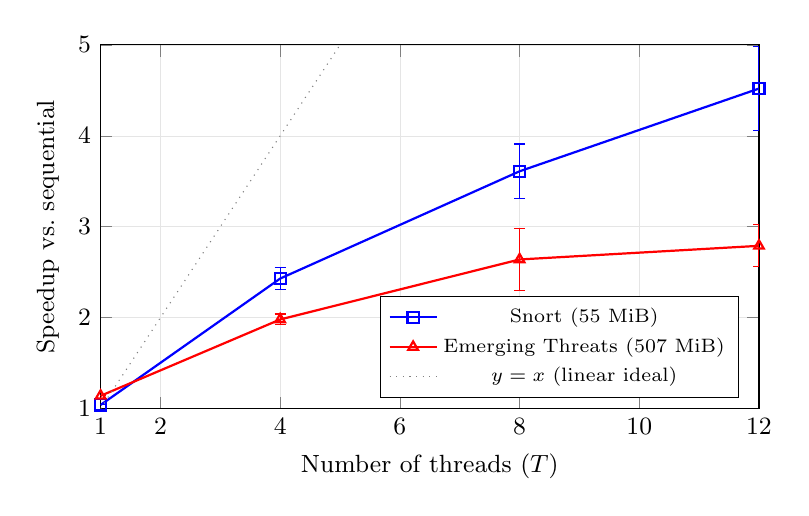
\begin{tikzpicture}
\begin{axis}[
    width=0.82\textwidth,
    height=6.2cm,
    xlabel={Number of threads ($T$)},
    ylabel={Speedup vs.\ sequential},
    xmin=1, xmax=12,
    ymin=1, ymax=5,
    xtick={1,2,4,6,8,10,12},
    ytick={1,2,3,4,5},
    legend pos=south east,
    legend style={font=\scriptsize},
    grid=both,
    grid style={line width=.1pt, draw=gray!10},
    major grid style={line width=.2pt, draw=gray!20},
    style={font=\small}
]
\addplot[color=blue, mark=square, thick, error bars/.cd, y dir=both, y explicit] coordinates {
    (1,1.04) +- (0,0.00) (4,2.43) +- (0,0.12) (8,3.61) +- (0,0.30) (12,4.52) +- (0,0.46)
};
\addlegendentry{Snort (55~MiB)}

\addplot[color=red, mark=triangle, thick, error bars/.cd, y dir=both, y explicit] coordinates {
    (1,1.14) +- (0,0.00) (4,1.98) +- (0,0.06) (8,2.64) +- (0,0.34) (12,2.79) +- (0,0.23)
};
\addlegendentry{Emerging Threats (507~MiB)}

\addplot[color=gray, dotted] coordinates {
    (1,1) (12,12)
};
\addlegendentry{$y=x$ (linear ideal)}
\end{axis}
\end{tikzpicture}
\label{fig:speedup}

{\footnotesize\raggedright \textbf{Source:} Prepared by the author.\par}
\end{figure}

% review: comment 052 -- describe the data first, then interpret it.
The two regimes behave differently. With the moderate dictionary, the best
text-parallel strategy rises steadily to $4.52\times$ at twelve threads
($1{,}087.1$~MB/s; CV~$10\%$); on the canonical corpus the dynamic-dispatch
strategy reaches $4.79\times$ ($1{,}148.1$~MB/s; CV~$2\%$), the highest search
speedup observed on the intrusion-detection-scale dictionaries. With the
memory-bound dictionary the curve flattens far earlier: the best strategy reaches
only $2.79\times$ at twelve threads (CV~$8\%$), and on the canonical corpus the
peak occurs near six threads ($2.85\times$; CV~$16\%$) before declining as more
threads are added. Both regimes scale sublinearly.

% review: comment 053 -- present the DRAM/bandwidth attribution as inference, not
% as a measured fact (no bandwidth or cache counters were instrumented).
The early plateau of the memory-bound regime is the central observation of this
experiment. Its most likely cause is contention for the shared memory bus: once
the automaton is about forty-two times the cache, adding threads---particularly
the slower Efficiency cores beyond the two Performance cores---no longer raises
throughput, which is consistent with the memory bus, rather than the core count,
being the binding resource. This remains an inference drawn from the shape of the
scaling curves and their agreement with the footprint experiment, not a direct
measurement: memory bandwidth and cache counters were not instrumented, a
limitation revisited in the discussion of threats to validity.

% review: comment 053; task step 7 -- the serial fraction is reported as an
% effective, observed quantity on the i5, not as a pure algorithmic constant.
In the moderate-dictionary regime, where bandwidth is not the binding constraint,
the $4.52\times$ ceiling at twelve threads is consistent with Amdahl's
law~\cite{Grama2003}: the observed $37.7\%$ parallel efficiency corresponds to an
effective serial fraction of roughly $15\%$. On this hybrid platform that fraction
is best read as an effective, observed quantity rather than a fixed algorithmic
constant, because it conflates genuine serialization (merge coordination and work
dispatch), the P/E asymmetry of the pool---in which the four Performance-core
hardware threads carry more per-thread weight than the eight Efficiency
cores---and residual memory contention. Parallel efficiency
(Eq.~\ref{eq:efficiency}) makes the contrast explicit: at twelve threads the
moderate regime achieves $37.7\%$ efficiency ($4.52\times / 12$) against $23.3\%$
($2.79\times / 12$) for the memory-bound regime. That this gap mirrors the
cache-residency difference far more than the per-thread synchronization cost is
why it is attributed here primarily to memory behaviour rather than to threading
overhead---again as an inference consistent with the footprint result, not a
counter-level measurement.

The local conclusion is that text parallelism delivers a sublinear but substantial
speedup whose ceiling is set by the footprint regime: useful and robust where the
working set is moderate, and bounded by memory behaviour once the automaton is much
larger than the cache. This confirms the sublinear-scaling hypothesis and sharpens
it, by tying the ceiling to the automaton footprint rather than to the number of
cores.

A separate experiment fixed the dictionary and strategy while changing the
corpus, to confirm that the text content is not the main factor.
The sequential throughput on the two corpora is nearly identical
($241.0$~MB/s versus $248.4$~MB/s), and the twelve-thread speedup is of the
same order on both ($4.42\times$ on the e-mail corpus versus $3.66\times$ on the
encyclopedic corpus). The apparent gap, however, is not statistically
distinguishable: the e-mail measurement carries a coefficient of variation of
roughly $66\%$, so the two figures overlap within run-to-run variation and the
difference should not be read as a genuine corpus effect. Because Aho-Corasick performs one transition per input
byte regardless of match density, the footprint of the automaton dominates the
behaviour far more than the characteristics of the corpus.

\subsecao{The Flattened Output Layout}

The proposed output-layout optimization replaces the pointer-chasing emission of
matches with a sequential read of a contiguous array. Because it changes only
the memory layout, its effect can be measured in isolation on a single thread.
% review: task step 8 -- report the regime dependence as observed on the i5, not
% as a universal growth law.
Table~\ref{tab:flat} shows that, on the i5, the gain is regime-dependent and
increases with memory pressure.

\begin{table}[H]
    \centering
    \caption{Single-threaded gain of the flattened output layout, by regime.}
    \label{tab:flat}
    \small
    \begin{tabular}{@{} l r r r r @{}}
        \toprule
        \textbf{Regime (dictionary)} & \textbf{Automaton} & \textbf{Baseline} & \textbf{Flattened} & \textbf{Gain} \\
         & & \textbf{(MB/s)} & \textbf{(MB/s)} & \\
        \midrule
        Snort-100 ($\ll$L3)      & 1.93~MiB   & 483.1 & 488.1 & $+1.0\%$ \\ \addlinespace
        Snort (full, $>$L3)      & 55.23~MiB  & 240.7 & 252.0 & $+4.7\%$ \\ \addlinespace
        Emerging Threats ($\gg$L3) & 506.78~MiB & 125.6 & 142.0 & $+13.0\%$ \\
        \bottomrule
    \end{tabular}

    {\footnotesize\raggedright \textbf{Source:} Prepared by the author. Single thread.\par}
\end{table}

When the automaton fits in cache, the optimization provides almost no
benefit ($+1.0\%$), because the linked structures are already cache-resident.
When the automaton is far larger than the cache, the contiguous layout avoids
the scattered misses of the pointer walk and delivers $+13.0\%$ on a single
thread, which is the cheapest gain available in the memory-bound regime. In the
parallel case, the layout is inherited by the chunked strategies, and the
flattened variants lead or tie their pointer-chasing counterparts in both intrusion-detection-scale regimes; the best results --- $4.52\times$ for the moderate dictionary at the multi-gigabyte scale and $2.85\times$ at the peak of the memory-bound regime on the canonical corpus --- come from strategies that incorporate this layout. It is
worth noting that the gain does not compound multiplicatively with text
parallelism in the moderate regime: there, the DRAM stalls of the transition
table already partially mask the emission cost, so the layout provides a smaller
improvement than its single-threaded figure would suggest. The optimization
is therefore best described as a cheap, broadly applicable improvement whose
payoff is largest exactly where the problem is hardest. On the i5 this payoff
increases with the automaton footprint; the precise progression of the gain is
platform-dependent, so the qualitative pattern---a larger benefit under heavier
memory pressure---is more robust than the specific per-regime percentages.

\subsecao{Load Balancing on Heterogeneous Cores}

On the hybrid processor, uniformly sized text segments create stragglers: the
threads assigned to Efficiency cores finish later than those on the faster
Performance cores, and the early finishers idle at the barrier. The effect is
visible not in the mean throughput but in its stability across repetitions.
Figure~\ref{fig:load_balancing} illustrates the three partitioning policies:
uniform chunking leaves the Performance-core thread idle at the barrier while the
Efficiency-core thread finishes, whereas frequency-weighted sizing and dynamic
dispatch equalize finishing times.


\begin{figure}[H]
\centering
\caption{Partitioning policies on heterogeneous cores: (a) static homogeneous
chunking leaves the faster Performance core idle at the barrier (stragglers);
(b) topology-aware, frequency-weighted chunking sizes each segment to its core's
speed; (c) dynamic dispatch hands out small tasks on demand. Both (b) and (c)
equalize finishing times.}

\includegraphics[width=0.78\linewidth]{load_balancing.pdf}
\par\smallskip
{\footnotesize\raggedright \textbf{Source:} Prepared by the author.\par}
\label{fig:load_balancing}
\end{figure}

Table~\ref{tab:balance} reports, for the canonical workload at twelve threads,
the coefficient of variation of the per-iteration timing.

\begin{table}[H]
    \centering
    \caption{Run-to-run stability of the text-parallel strategies (twelve threads).}
    \label{tab:balance}
    \small
    \begin{tabular}{@{} l r r @{}}
        \toprule
        \textbf{Strategy} & \textbf{Throughput (MB/s)} & \textbf{Variation (CV)} \\
        \midrule
        Static homogeneous chunking            & 1{,}064.7 & $39.9\%$ \\ \addlinespace
        Static chunking (cache-padded)         & 902.0     & $52.9\%$ \\ \addlinespace
        Topology-aware (frequency-weighted)    & 879.8     & $1.7\%$  \\ \addlinespace
        Dynamic dispatch                       & 864.4     & $3.3\%$  \\ \addlinespace
        Flattened output with chunking         & 1{,}007.2 & $0.4\%$  \\ \addlinespace
        Topology-aware with flattened output   & 994.2     & $4.3\%$  \\
        \bottomrule
    \end{tabular}

    {\footnotesize\raggedright \textbf{Source:} Prepared by the author. Canonical workload, twelve threads; dedicated stability diagnostic (three timed iterations under sustained load). The mean throughputs are subject to the run-to-run variance the table quantifies and are not directly comparable with the sustained figures of the scalability analysis.\par}
\end{table}

The static homogeneous strategies exhibit a coefficient of variation between
$39.9\%$ and $52.9\%$, consistent with slower cores intermittently delaying the
overall execution. Both
solutions proposed in the design reduce this variation: frequency-weighted
partitioning reduces it to $1.7\%$ and dynamic dispatch to $3.3\%$, while the
flattened chunking strategy is the most stable of all (down to $0.4\%$) --- indicating that uniform partitioning makes the run-to-run timing sensitive to how the scheduler places the slow-core segments, rather than imposing a fixed penalty. This shows that topology awareness does not make the transition function faster;
it removes idle time at the barrier, trading a small change in
mean throughput for a large gain in predictability. The improvement is in
predictability and worst-case latency, not in mean throughput, and it does not by
itself change the ranking of strategies, because the underlying ceiling remains
the memory subsystem.
% review: task step 9 -- mark topology-aware balancing as specific to hybrid
% hardware; separate predictability from mean throughput.
Because the stragglers arise from the Performance/Efficiency split of this
processor, this is a result specific to hybrid CPUs such as the i5: on a
homogeneous machine, uniformly sized segments would not produce the same
imbalance, and topology-aware sizing would have little to correct. The value
demonstrated here is therefore the decoupling of timing predictability from mean
throughput on heterogeneous cores, rather than a universal throughput gain.

\subsecao{Parallel Construction of the Automaton}

The construction phase can also be parallelized, because each level of the
breadth-first traversal that computes the failure links depends only on shallower
levels and can therefore be processed in parallel with a barrier between levels.
The trie insertion remains sequential; only the traversal is parallelized.
Figure~\ref{fig:parallel_bfs} sketches the dependency structure: failure links at
a given level read only links from shallower levels, so the threads computing a
level can run concurrently and synchronize at a barrier before the next level
begins.


\begin{figure}[H]
\centering
\caption{Level-synchronous parallel construction of the failure function. Threads
compute the failure links of all states at one BFS level in parallel, reading
only already-finalized links from shallower levels (green), and meet at a barrier
before advancing to the next level.}

\includegraphics[width=1.0\linewidth]{parallel_bfs.pdf}
\par\smallskip
{\footnotesize\raggedright \textbf{Source:} Prepared by the author.\par}
\label{fig:parallel_bfs}
\end{figure}

Table~\ref{tab:build} reports the build speedup across thread counts, rather than
a single peak, so that the full thread-count behaviour is visible.

% review: comment 057 -- show the build speedup at each thread count instead of
% only the per-dictionary peak.
\begin{table}[H]
    \centering
    \caption{Parallel automaton construction: build speedup versus the sequential
    build, by thread count.}
    \label{tab:build}
    \small
    \begin{tabular}{@{} l r r r r r r @{}}
        \toprule
        \textbf{Dictionary} & \textbf{States} & \textbf{Seq.\ (ms)} & \textbf{$T{=}2$} & \textbf{$T{=}4$} & \textbf{$T{=}8$} & \textbf{$T{=}12$} \\
        \midrule
        Snort-100        & 1{,}939   & 1.5   & $0.80\times$ & $0.83\times$ & $0.71\times$ & $0.60\times$ \\ \addlinespace
        Snort (full)     & 55{,}479  & 48.2  & $1.00\times$ & $1.19\times$ & $1.17\times$ & $0.91\times$ \\ \addlinespace
        Emerging Threats & 508{,}896 & 485.2 & $1.18\times$ & $1.43\times$ & $1.55\times$ & $1.41\times$ \\
        \bottomrule
    \end{tabular}

    {\footnotesize\raggedright \textbf{Source:} Prepared by the author. Build
    speedup is the sequential build time divided by the parallel build time at
    each thread count; values below $1.0\times$ mean the parallel build is slower
    than the sequential one.\par}
\end{table}

The thread-count breakdown shows that parallel construction only pays off for the
large dictionary, where it peaks at $1.55\times$ at eight threads (reducing the
build from $485$ to roughly $313$~milliseconds) before easing to $1.41\times$ at
twelve. The moderate dictionary barely benefits, peaking at $1.19\times$ at four
threads and regressing to $0.91\times$ at twelve, while the smallest dictionary is
slower than sequential at every thread count, because the per-level
spawn-and-join overhead exceeds the work. This optimization should therefore be
understood as an operational benefit---a reduction in rule-reloading latency for
systems that frequently update their signatures---rather than as a contribution to
scanning throughput; on the multi-gigabyte workloads it accounts for less than
$1\%$ of the total time.

\subsecao{Partitioning the Dictionary: A Qualified Negative Result}

Partitioning the dictionary, rather than the text, was evaluated as an alternative,
assigning patterns to shards by their first byte (prefix sharding).
Table~\ref{tab:shard} reports the throughput across shard counts and compares the
result against plain text parallelism on the canonical workload.

% review: comment 058 -- the data points discussed in the text (the two-shard
% figure and the saturation past the peak) are now in the table itself.
\begin{table}[H]
    \centering
    \caption{Dictionary sharding (by prefix) across shard counts, compared to text
    parallelism (Snort, canonical corpus).}
    \label{tab:shard}
    \small
    \begin{tabular}{@{} l r r @{}}
        \toprule
        \textbf{Configuration} & \textbf{Throughput (MB/s)} & \textbf{vs.\ sequential} \\
        \midrule
        Prefix sharding, 2 shards          & 322.6 & $1.35\times$ \\ \addlinespace
        Prefix sharding, 4 shards          & 319.9 & $1.34\times$ \\ \addlinespace
        Prefix sharding, 6 shards (peak)   & 327.2 & $1.37\times$ \\ \addlinespace
        Prefix sharding, 8 shards          & 291.3 & $1.22\times$ \\ \addlinespace
        Prefix sharding, 12 shards         & 276.6 & $1.15\times$ \\
        \midrule
        Text chunking, flat (12 threads)   & 976.1 & $4.07\times$ \\
        \bottomrule
    \end{tabular}

    {\footnotesize\raggedright \textbf{Source:} Prepared by the author. Speedup is relative to the single-threaded sequential baseline ($239.6$~MB/s); text chunking is shown at twelve threads for reference.\par}
\end{table}

Prefix sharding peaks at $1.37\times$ over the baseline at six shards, but it is
already within $2\%$ of that peak at just two shards ($1.35\times$) and declines
past six. This early saturation indicates that the benefit comes from improved
cache locality within each smaller sub-automaton rather than from added
parallelism. Even at its best it attains only about a third ($0.34\times$) of the
throughput of plain text parallelism. The conclusion is that, on this class of
hardware, partitioning the text dominates partitioning the dictionary: a real but
small effect, not a competitive strategy.

% review: comment 059 -- more descriptive section title.
\subsecao{Combined Strategy Evaluation: Sharding with Chunking}

A natural hypothesis is that combining dictionary sharding (for cache locality)
with text chunking (for parallelism) would recover the throughput lost in the
memory-bound regime, by making each sub-automaton small enough to approach the
cache. Table~\ref{tab:twod} tests this two-dimensional composition against flat-output
text chunking and disproves the hypothesis.

\begin{table}[H]
    \centering
    \caption{Two-dimensional composition versus flat-output text chunking (twelve threads).}
    \label{tab:twod}
    \small
    \begin{tabular}{@{} l r r r @{}}
        \toprule
        \textbf{Workload} & \textbf{Composition} & \textbf{Text chunking} & \textbf{Ratio} \\
         & \textbf{(MB/s)} & \textbf{(MB/s)} & \\
        \midrule
        Snort, canonical corpus              & 785.4 & 976.1 & $0.80\times$ \\ \addlinespace
        Snort, $\sim$10.6~GiB                & 861.6 & 1{,}073.3 & $0.80\times$ \\ \addlinespace
        Emerging Threats, canonical corpus   & 289.0 & 312.3 & $0.93\times$ \\ \addlinespace
        Emerging Threats, $\sim$10.6~GiB     & 314.5 & 350.0 & $0.90\times$ \\
        \bottomrule
    \end{tabular}

    {\footnotesize\raggedright \textbf{Source:} Prepared by the author. Twelve threads in both columns; the comparator is the flat-output text chunking of Table~\ref{tab:shard}.\par}
\end{table}

The composition is slower than flat-output text chunking in every measured scenario,
by $7\%$ to $20\%$. The reason is that each shard must scan the entire
input text, so $K$ shards multiply the text traffic on the memory bus by a factor
of $K$. In the memory-bound regime that traffic is already the bottleneck, so
the extra reads outweigh any locality gained inside the smaller sub-automata. To
shrink the sub-automaton below the last-level cache for the largest dictionary
would require more than forty shards, multiplying the text traffic
proportionally, which is unrecoverable on a memory bus of this bandwidth. This
negative result is an important contribution: it closes a plausible region of
the design space and reinforces the conclusion that text parallelism is the
correct axis on memory-bound workloads. This difference in memory traffic is illustrated in Figure~\ref{fig:memory_traffic}.

% review: comment 060 -- this explanatory figure belongs in the proposal chapter;
% its relocation (and the accompanying strategy explanation) is owned by
% epic-02 task-02 and is left in place here pending that move.
\begin{figure}[H]
\centering
\caption{Visual comparison of text reading traffic: (a) pure text chunking (text parallelism) where each byte is read once, keeping bus load moderate; and (b) two-dimensional composition (chunking + sharding) which multiplies the text reads by $K$ shards, saturating the DRAM bus and degrading speedup.}

\includegraphics[width=0.9\linewidth]{memory_traffic.pdf}
\par\smallskip
{\footnotesize\raggedright \textbf{Source:} Prepared by the author.\par}
\label{fig:memory_traffic}
\end{figure}

% review: comment 061 -- this section does not pose a new experimental question;
% it is reframed as a consistency check that confirms, rather than extends, the
% separate construction and search analyses at the level of the whole pipeline.
\subsecao{End-to-End Consistency Check}

The preceding sections measured construction and search in isolation. This final
check verifies that those results hold for the complete pipeline---automaton
construction followed by a single full scan of the $\sim$10.6~GiB corpus, reported
as wall-clock time. It introduces no new experiment: to keep the figures
auditable, each cell is reconstructed from the same canonical sweep as the
measured build time plus one full-corpus search pass (Table~\ref{tab:e2e}).

\begin{table}[H]
    \centering
    \caption{End-to-end wall-clock on the $\sim$10.6~GiB corpus, as construction
    time plus a single full-corpus scan.}
    \label{tab:e2e}
    \small
    \begin{tabular}{@{} l r r r @{}}
        \toprule
        \textbf{Dictionary} & \textbf{Sequential (ms)} & \textbf{Best parallel (ms)} & \textbf{Speedup} \\
        \midrule
        Snort (full)     & 45{,}174  & 10{,}027 & $4.50\times$ \\ \addlinespace
        Emerging Threats & 86{,}998  & 31{,}517 & $2.76\times$ \\
        \bottomrule
    \end{tabular}

    {\footnotesize\raggedright \textbf{Source:} Prepared by the author, derived
    from the 2026 canonical sweep. Each cell is the measured build time plus one
    full-corpus search pass ($\textit{build\_ms} + \textit{mean\_ms}$); the
    parallel column uses the best twelve-thread strategy with a sequential
    build.\par}
\end{table}

The end-to-end speedups are $4.50\times$ for the moderate dictionary (roughly
forty-five seconds down to ten) and $2.76\times$ for the memory-bound one ($87.0$
to $31.5$~seconds, with flat-output text chunking and a sequential build).
Because construction accounts for under one percent of the pipeline---$49$~ms of
$45{,}174$~ms for Snort and $541$~ms of $86{,}998$~ms for Emerging Threats---these
figures track the search-only speedups of Figure~\ref{fig:speedup} almost exactly
($4.50\times$ versus $4.52\times$; $2.76\times$ versus $2.79\times$). The pipeline
is therefore dominated by the scanning phase, and the end-to-end measurement adds
no scaling beyond what the search analysis already establishes; it serves only to
confirm that the earlier speedups hold end to end.

\subsecao{Discussion and Positioning}

% review: comment 062 -- soften the over-confident framing; the i5 results give a
% consistent reading, and the memory-bandwidth shift is stated as a consistent
% inference rather than a measured cause.
Taken together, the i5 results converge on a consistent reading. On this platform,
the dominant obstacle to accelerating Aho-Corasick at intrusion-detection scale
appears to be microarchitectural: once the automaton greatly exceeds the
last-level cache, performance is bounded by the memory subsystem, and the most
effective response is to parallelize the text while keeping the per-byte
transition cost as low as possible. No single strategy is best across all regimes;
the fastest strategy switches between dynamic dispatch (moderate dictionary on the
canonical corpus) and the flattened variants, with and without topology awareness,
in the remaining scenarios. This pattern is consistent with the main bottleneck
shifting, as the dictionary grows, from thread scheduling toward memory
bandwidth---the regime in which a cache-friendly emission path helps the most---an
interpretation inferred from the measurements rather than confirmed by
hardware-counter instrumentation.

These findings can be positioned against the related literature. Compared to
approaches that restructure the automaton to improve cache friendliness,
such as the head--body decomposition of the matcher for multi-core intrusion
detection~\cite{LeeYang2017FHBM}, the present work attains a comparable order of
magnitude of throughput while leaving the classical automaton mathematically
intact, which keeps correctness easy to validate against the sequential
reference. The failure-less variant of the algorithm designed for massively
parallel accelerators~\cite{Vajira2018} is, however, unsuitable for a
multi-core CPU, because its independent per-byte traversals multiply work in a
way that the memory bus cannot absorb; this is consistent with the negative
result observed here for over-partitioning. Single-threaded vectorized engines
that replace the automaton with SIMD literal matching~\cite{Xu2023Harry} operate
on an orthogonal axis, exploiting data parallelism within a thread rather than
across threads, and are therefore complementary to, rather than competitive with, the inter-thread parallelism studied here. The finding that
layout-level changes to the emission path yield real gains aligns with work on
transition-table compression for the same algorithm~\cite{Regeciova2021MYARA}.
Finally, the use of realistic rule sets and large corpora follows the guidance on
representative signature-based intrusion-detection benchmarks~\cite{Aldwairi2018Characterizing},
which is what allows the memory-bound regime to be studied, rather than an artificially
cache-friendly one.
